\subsection{Storage Structure and Memory Hierarchy}

A CPU can load instructions only from memory.
Main memory is rewritable RAM --- commonly implemented with DRAM semiconductor technology.

Memory is an array of bytes.
Each byte has its own address.
Bytes are moved between memory and CPU registers with load and store instructions.
The CPU automatically loads instructions from main memory for execution.

The fetch instruction loads an instruction from memory.
When the instruction is decoded, operands may also be loaded from memory.
After the instruction is executed, the result is stored to memory.
The memory unit only sees a stream of addresses.

Ideally, both program instructions and data would reside in the main memory.
However, this is difficult as main memory is small and volatile (erased after loss of power).
The solution is to store programs and data in secondary storage.
When programs are run, their instructions are loaded from secondary storage to main memory.

There are many forms of storage available.
They differ in speed, cost, size and volatility.

\begin{table}[htp]
  \centering
  \caption*{Typical properties of storage types.}
  \begin{tabular}{rlrrrll}
    \toprule
    Level & Name & Size & Access time / \si{\nano\second} & Bandwidth / \si{\mebi\byte\per\second} & Managed by \\
    \midrule
    1 & Registers & \( < \SI{1}{\kibi\byte} \) & \numrange{0.25}{0.5} & \numrange{20000}{100000} & Compiler \\
    2 & Cache & \( < \SI{16}{\mebi\byte} \) & \numrange{0.5}{25} & \numrange{5000}{10000} & Hardware \\
    3 & Main memory & \( < \SI{64}{\gibi\byte} \) & \numrange{80}{250} & \numrange{1000}{5000} & OS \\
    4 & Solid-state disk & \( < \SI{1}{\tebi\byte} \) & \numrange{25000}{50000} & \num{500} & OS \\
    5 & Magnetic disk & \( < \SI{10}{\tebi\byte} \) & \num{5000000} & \numrange{20}{150} & OS \\
    \bottomrule
  \end{tabular}
\end{table}

\subsubsection{Memory}

Memory is an array of bytes, in which each byte is addressable.ROM cannot be modified.
EEPROM can be modified, but only infrequently.
The CPU requires memory that can be read and written.
It uses dynamic RAM (DRAM) and registers.

Main memory is erased when a machine powers off.
Secondary storage is used as a more permanent solution.
This includes magnetic and optical disks.

Data that is used frequently is stored in cache memory for faster access.
If the CPU requires data, the cache is checked first.
\begin{figure}[htp]
  \centering
  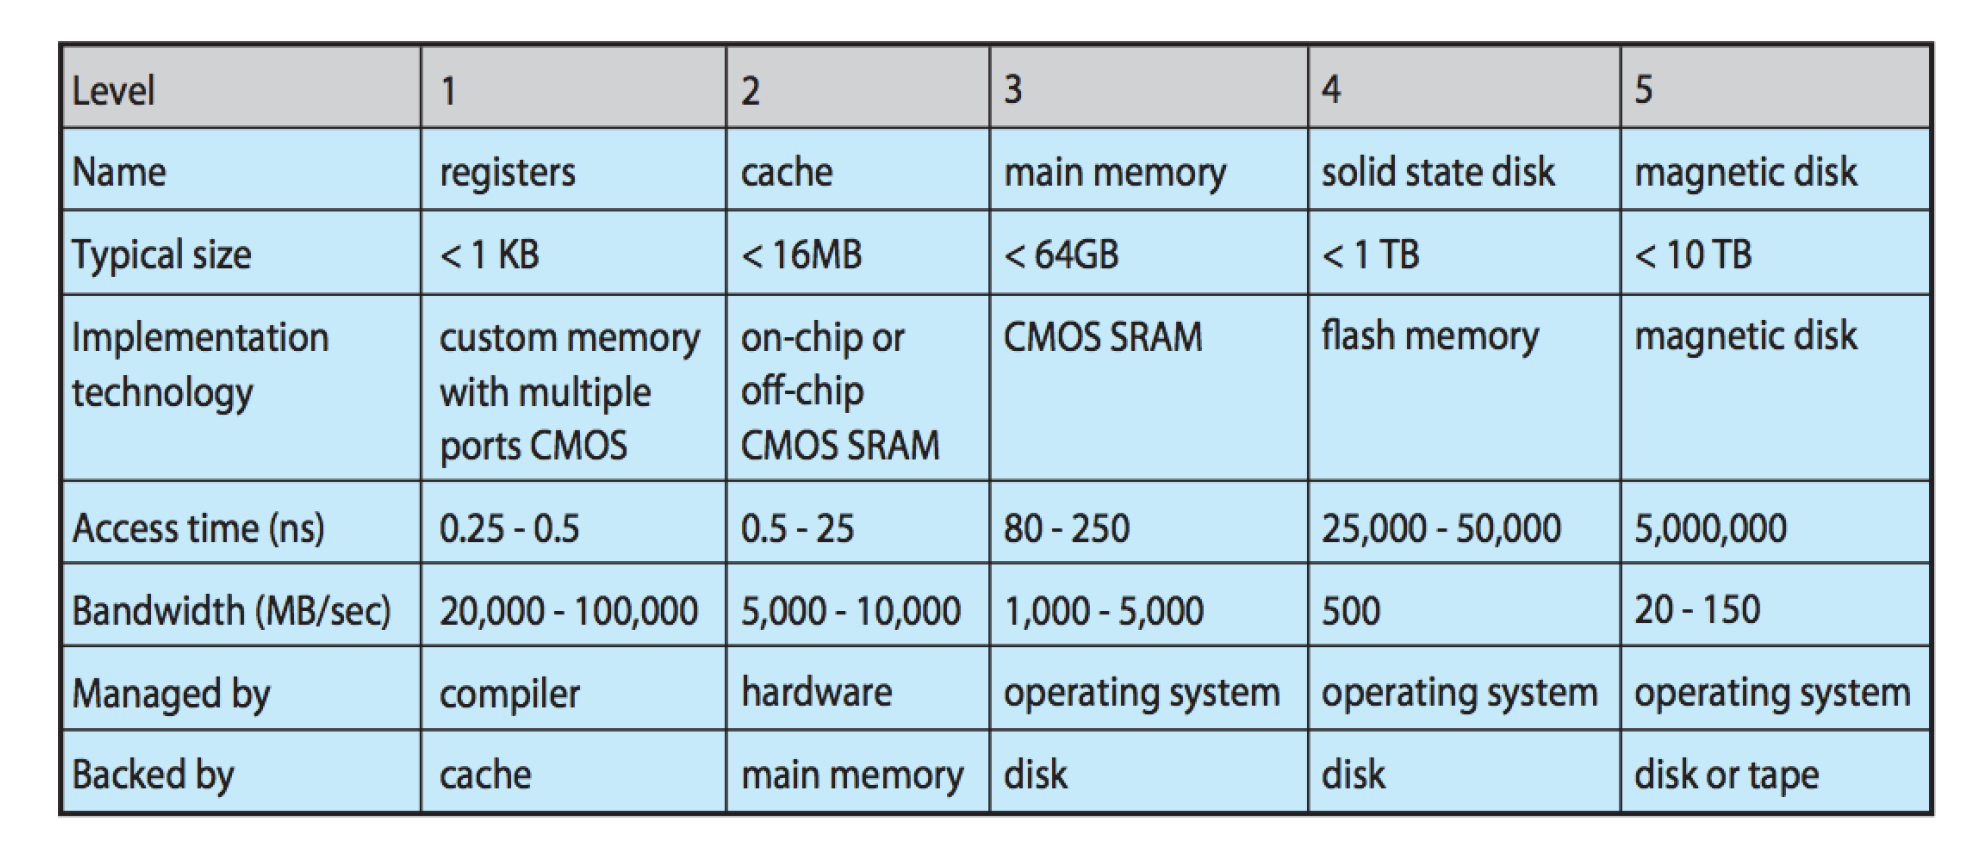
\includegraphics[width=12cm]{unit-7/figures/01.png}
  \caption*{Storage Comparison}
\end{figure}
\subsection{I/O Structure}

A large portion of OS code is dedicated to the management of I/O\@.
Without I/O, computers would be useless.
The hardwares may trigger an interrupt at any time by sending a signal to the CPU.
An I/O device interacts with the system via a `device controller' connected through a common bus to the CPU\@.
\newline
A small computer system interface (SCSI) controller is a piece of hardware that allows an SCSI storage device to communicate with the operating system via an SCSI bus.
A device controller maintains some local buffer storage and a set of special-purpose registers.
The device controller moves data between the peripheral device it controls and its local buffer storage.
\newline
An OS has a device driver for each device controller.
These are typically downloaded.
The device driver is able to interact with its corresponding device controller and provides the OS with a uniform interface to the device.
\begin{figure}[htp]
  \centering
  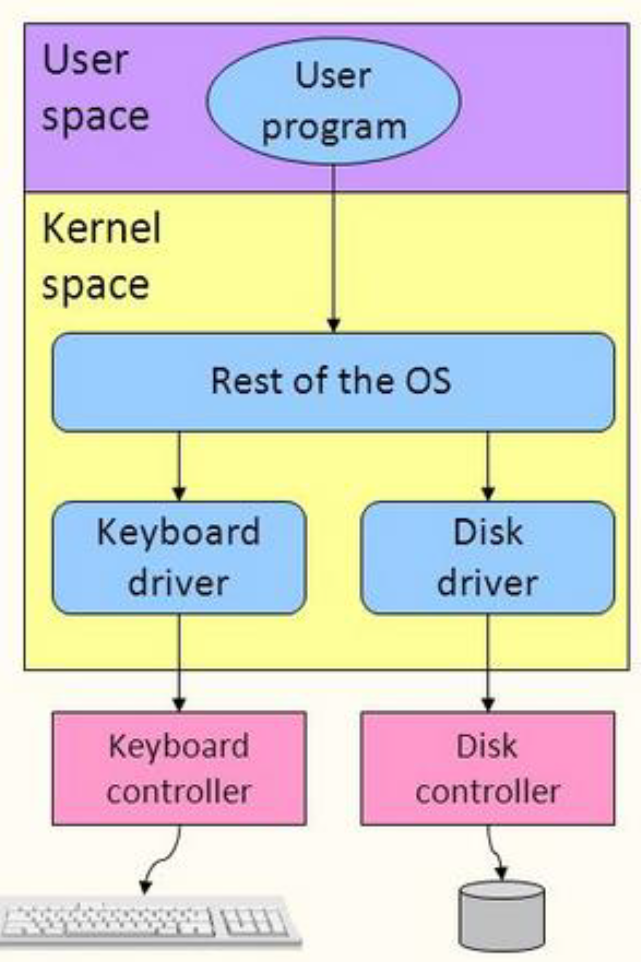
\includegraphics[width=12cm]{unit-7/figures/02.png}
  \caption*{Storage Comparison}
\end{figure}
\subsection{I/O Mechanisms}
There are three types of I/O mechanism.
\begin{enumerate}
  \item Programmed I/O (also known as `polling')
  \item Interrupt-driven I/O
  \item Direct memory access (DMA)
\end{enumerate}
\subsubsection{Programmed I/O}

Programmed I/O requires the CPU to `poll' the status of the controller by repeatedly checking its status until it is ready to accept an I/O request.
It then continues to check the status of the controller until the I/O operation is complete.
\newline
This mechanism is very fast due to the direct involvement of the CPU\@.
However, this also prevents the CPU from working on other tasks that may be more important.
\newline
The processor has special instructions that control I/O device ,test status and transfer of data (read/write)
However the performance Issue is the processor is busy checking the I/O status of the I/O module.
\subsubsection{Interrupt-Driven I/O}

Interrupt driven I/O works as follows.
\begin{enumerate}
  \item The CPU initiates I/O through the device driver.
  \item The CPU checks for interrupts between executing other instructions.
  \item The device controller begins the I/O operation.
  \item When input is ready, output is complete or there is an error, the device controller sends an interrupt signal to the CPU.
  \item When the CPU detects the interrupt, control is transferred to the interrupt handler, which will process the data before returning from the interrupt.
  \item The CPU resumes the interrupted task.
\end{enumerate}
Interrupt driven I/O is suitable for transferring small amounts of data.
The CPU is less involved in the I/O operation and is free to execute other instructions.
However, this reduces the speed of the I/O operation.

\subsubsection{Direct Memory Access (DMA)}

The DMA controller transfers data directly between the I/O device and memory.
This requires additional architecture for the device, including buffers, pointers and counters.
The device controller transfers entire blocks of data to and from its own buffer storage and memory.
There is no direct involvement of the CPU during transfer.
\begin{enumerate}
  \item The CPU programs the DMA controller.
  \item The DMA controller requests transfer to memory.
  \item The disk controller transfers the data to memory.
  \item The disk controller checks with the DMA controller that there is no more data to transfer.
  \item The DMA controller sends an interrupt signal to the CPU when transfer is complete.
\end{enumerate}

\begin{figure}[htp]
  \centering
  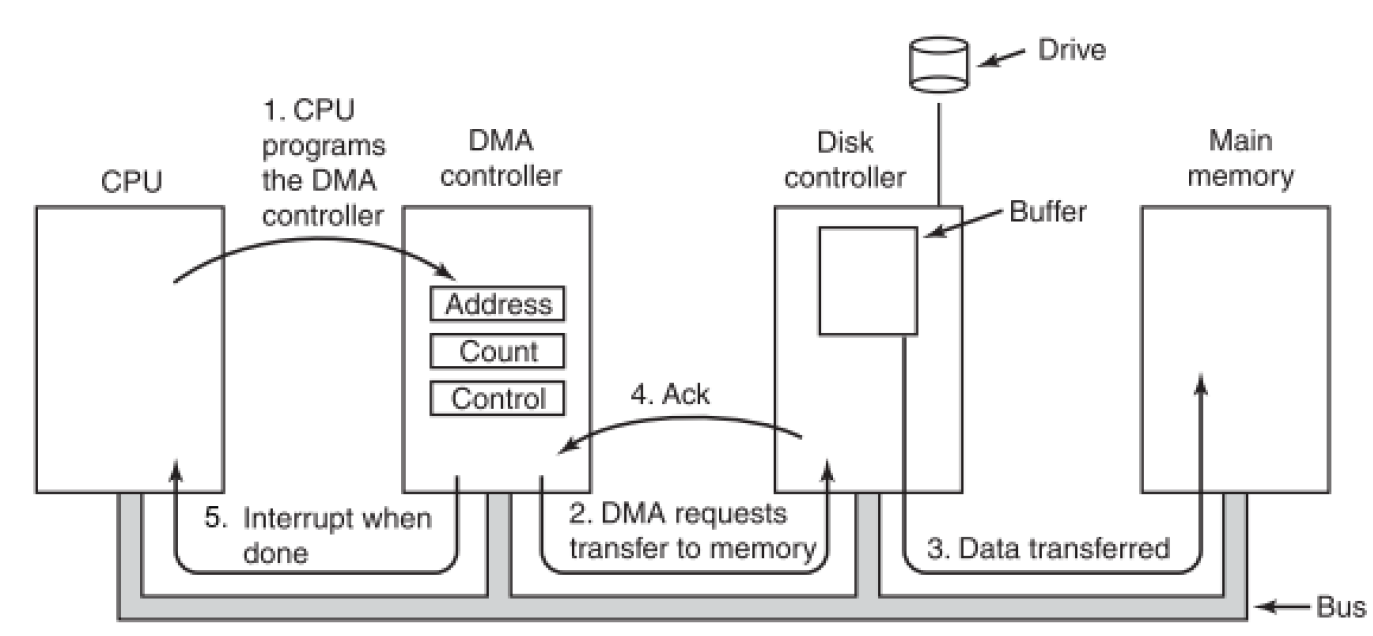
\includegraphics[width=12cm]{unit-7/figures/03.png}
  \caption*{Direct Memory Access}
\end{figure}
Only a single interrupt is generated.
This is much better than the one interrupt per byte generated by low-speed devices.
The CPU is completely free to execute other instructions.
However, both the DMA controller and the CPU share the bus that connects different hardware components.
Thus, the CPU will experience slowdown during DMA transfer as it must wait for access to the bus.

\subsubsection{Computer System Architecture}
Single-processor and multiprocessor systems. Single-processor systems have one CPU, sometimes including special-purpose processors. In contrast, multiprocessor systems, which include parallel and multicore setups, share the bus, clock, memory, and peripherals. These systems range from servers to smartphones and offer benefits such as increased throughput, improved cost efficiency, and better reliability through graceful degradation.
\pagebreak
\subsection{General Computer System Architectures}

\subsubsection{Multiprocessor Sytems}

Multiprocessor systems have multiple processors in parallel or multiple cores.
The processors share the bus, clock, memory and peripherals.
This increases throughput, although this does not increase linearly with the number of processors.
There is also an economy of scale, as additional processors share the same peripherals, storage and power.
Reliability is also increased, as a failed processor will not stop the entire system.
This is known as `graceful degradation'.

Asymmetric multiprocessor systems follow a boss-worker relationship.
Each processor is assigned a specific task.

Symmetric multiprocessor systems follow a peer-to-peer relationship.
Each processor is utilised and has an equal chance of being used.
\subsubsection{\sout{Non-Uniform Memory Access (NUMA)}}
\sout{
In non-uniform memory access (NUMA) systems, multiple processors are interconnected and each processor has its own memory.
Each processor can access the other memories through their corresponding processors, but this is slower than direct access to its own memory.
}
\subsubsection{\sout{Multicore Systems}}
\sout{
Multicore systems have multiple cores on a single chip.
This is useful because on-chip communication is faster and consumes less power.
This is used in blade servers to minimise physical space and power consumption.
}
\subsubsection{\sout{Clustered Systems}}
\sout{
Clustered systems incorporate multiple interconnected computers with a shared network storage.
This provides a high availability of computers and processors, which is useful if one computer fails.
It also facilitates standby or backup servers, high-performance computing and parallelisation of applications.
}
\subsection{Operating System Services}
Operating system installations typically include
\begin{itemize}
  \item system programs (program loader, command interpreter),
  \item language processors (C compiler, assembler, linker),
  \item utilities (text editor, terminal emulator), and
  \item subroutine libraries (standard C library, JVM).
\end{itemize}

\subsection{System Calls}

System calls provide OS services to the user via an application programming interface (API).
System calls APIs are typically written in C or C++, though some are written in assembly language.
System calls are mostly accessed by programs via a high-level Application Programming Interface (API) rather than direct system call use
Three most common APIs are Win32 API for Windows, POSIX API for POSIX-based systems (including virtually all versions of UNIX, Linux, and Mac OS X), and Java API for the Java virtual machine (JVM)
\newline
Typically, there is a number associated with each system call.
The system call interface maintains a table indexed according to these numbers.
The system call interface invokes the requested system call in the OS kernel and returns the status of the system call and any return values.
\newline
The system call for reading data from one file and writing it to another is \texttt{cp <file1> <file2>}.
This uses the following services.
\begin{itemize}
  \item Open \texttt{file1}
  \item Handle possible error
  \item Create \texttt{file2}
  \item Start read and write
  \item Handle possible errors
  \item Close \texttt{file1} and \texttt{file2}
\end{itemize}
The services are not accessed directly.
They are accessed via an API.

\begin{table}[htp]
  \centering
  \caption*{Examples of Windows and Unix system call APIs.}
  \begin{tabular}{lll}
    \toprule
    Type of call & Windows & Unix \\
    \midrule
    Process Control & \texttt{CreateProcess()}       & \texttt{fork()} \\
                    & \texttt{ExitProcess()}         & \texttt{exit()} \\
                    & \texttt{WaitForSingleObject()} & \texttt{wait()} \\
    File Manipulation & \texttt{CreateFile()}  & \texttt{open()}  \\
                      & \texttt{ReadFile()}    & \texttt{read()}  \\
                      & \texttt{WriteFile()}   & \texttt{write()} \\
                      & \texttt{CloseHandle()} & \texttt{close()} \\
    Device manipulation & \texttt{SetConsoleMode()} & \texttt{ioctl()} \\
                        & \texttt{ReadConsole()}    & \texttt{read()}  \\
                        & \texttt{WriteConsole()}   & \texttt{write()} \\
    Information maintenance & \texttt{GetCurrentProcessID()} & \texttt{getpid()} \\
                            & \texttt{SetTimer()}            & \texttt{alarm()}  \\
                            & \texttt{Sleep()}               & \texttt{sleep()}  \\
    Communication & \texttt{CreatePipe()}        & \texttt{pipe()}   \\
                  & \texttt{CreateFileMapping()} & \texttt{shmget()} \\
                  & \texttt{MapViewOfFile()}     & \texttt{mmap()}   \\
    Protection & \texttt{SetFileSecurity()}              & \texttt{chmod()} \\
               & \texttt{InitializeSecurityDescriptor()} & \texttt{umask()} \\
               & \texttt{SetSecurityDescriptorGroup()}   & \texttt{chown()} \\
    \bottomrule
  \end{tabular}
\end{table}

System call APIs specify a set of functions that are available to an application programmer.
They describe the parameters to pass to each function, and the values that are returned.
The programmer accesses the API via a library provided by the OS.

A Java API exists for programs that run on the JVM\@.
The JVM itself uses the system calls of its particular platform.

System call APIs are used for program portability.
A program using the API can be compiled and run on any system that supports the API\@.
Invoking system calls directly is usually more difficult.
Using a system call API is similar to implementing an interface.
\begin{figure}[htp]
  \centering
  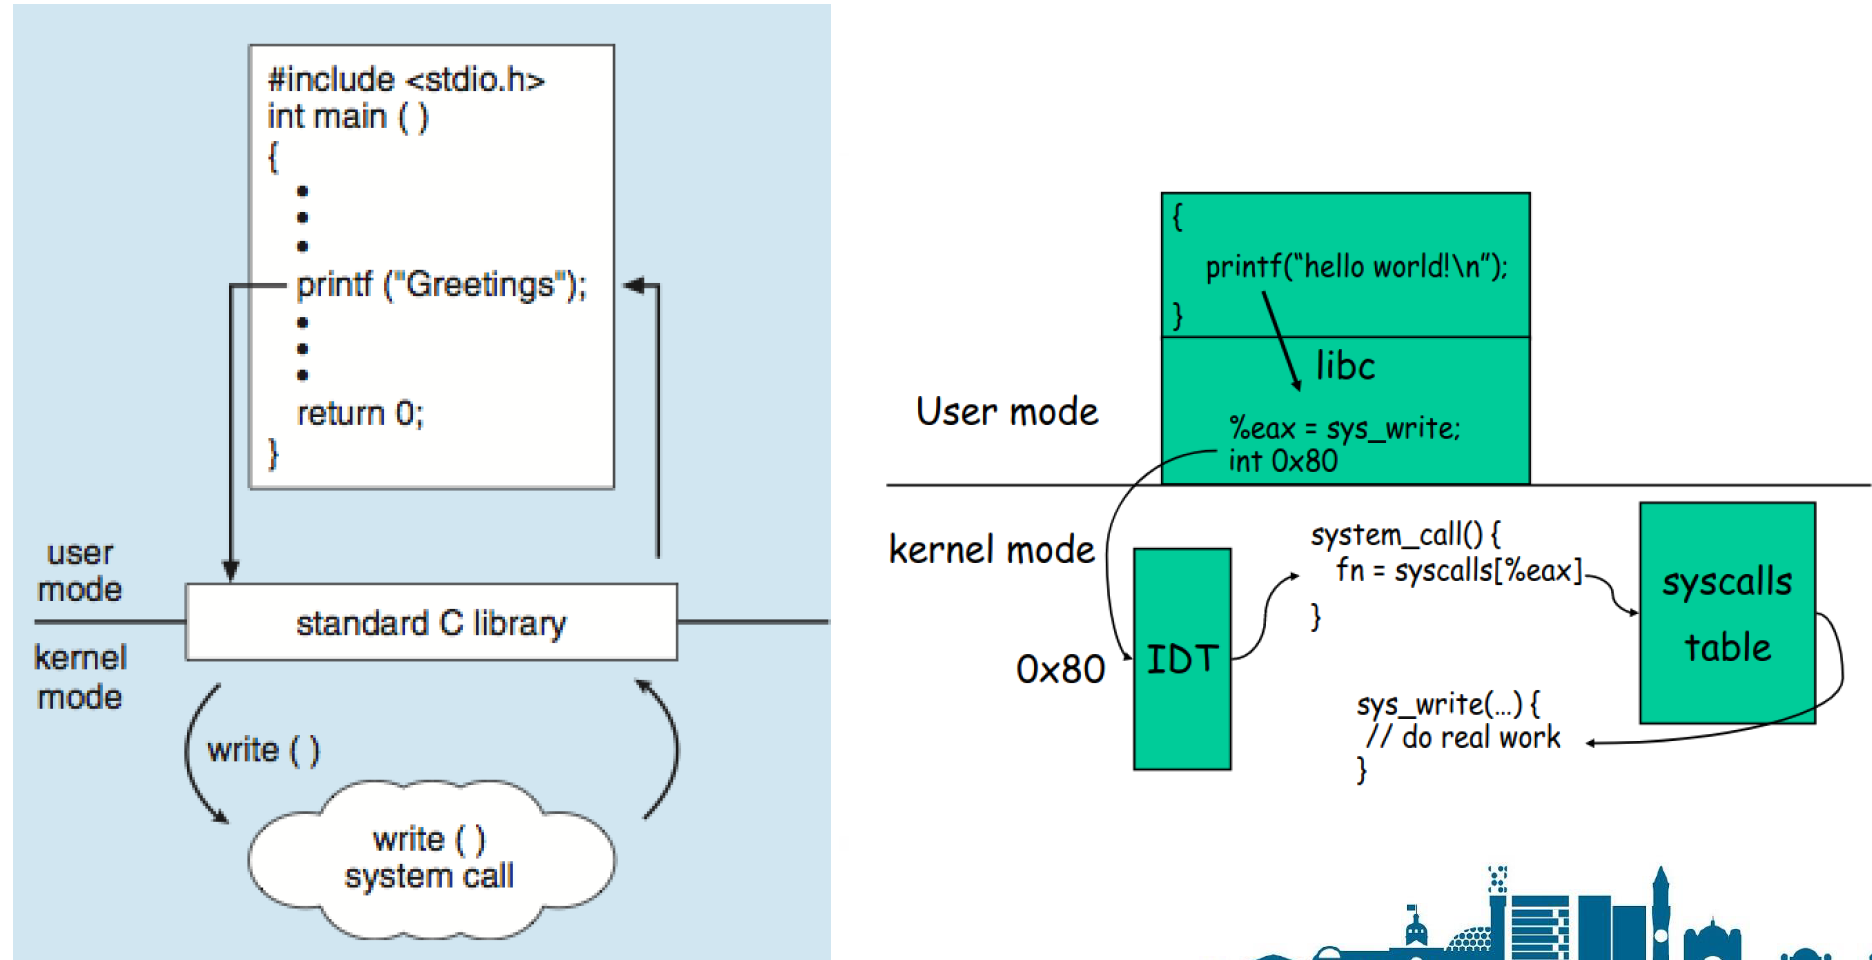
\includegraphics[width=12cm]{unit-7/figures/05.png}
  \caption*{Standard C Library Example}
\end{figure}
\subsection{Dual Mode}

Operating system execution is split into user mode (mode bit of value \num{1}) and kernel mode (mode bit of value \num{0}).
In user mode, certain areas of memory are protected from user access, and certain instructions cannot be executed.
In kernel mode, protected areas of memory may be accessed, and privileged instructions may be executed.

The OS allows user programs to execute system calls by resetting the mode bit to \num{0}.
Once the kernel has executed the requested system call, the mode bit is set to \num{1}.
This prevents crashes in user mode from affecting the kernel.

The MS-DOS architecture has no mode bit.
Hence, user programs were able to wipe the entire OS, write to devices without permission, execute illegal instructions and access the memory of other users.
\newline
With dual mode, hardware can stop user program attempting to execute an illegal instruction or to access memory of other users.
\newline
When a mode violation is detected, the OS must terminate the program, give an error message and produce memory dumps by writing to a file.
\begin{figure}[htp]
  \centering
  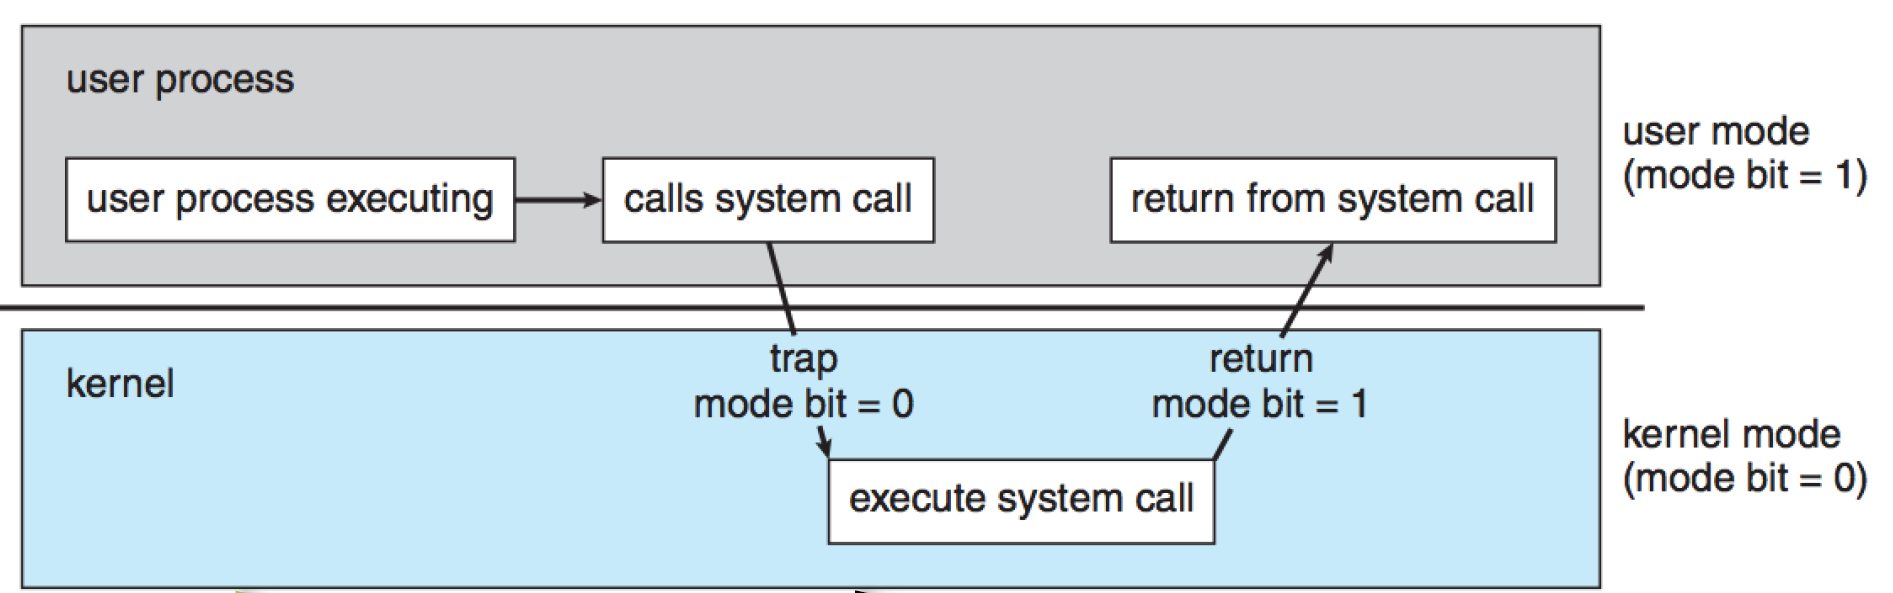
\includegraphics[width=12cm]{unit-7/figures/04.png}
  \caption*{Dual Mode}
\end{figure}
\subsection{OS Design and Implementation}

The internal structures of operating systems can vary widely.
The goals and specifications of an OS can be affected by hardware and the type of system.
User goals are that the OS should be convenient to use, easy to learn, reliable, safe and fast.
System goals are that the OS should be easy to design, implement and maintain, as well as flexible, reliable, error-free and efficient.

Early operating systems were produced in assembly language, then in system programming languages such as Algol and PL/I\@.
Nowadays they are written in C and C++.

Modern operating systems actually use a combination of different languages.
The lowest levels may be written in assembly, the main body in C, and system programs in C, C++, PERL, Python and shell scripts.
Operating systems written in higher-level languages are easier to port to other hardware, but they are also slower.
Emulation allows an OS to run on non-native hardware.

\subsection{Operating System Structure}

A general-purpose OS is a very large program.
There are various ways to structure one.
\begin{itemize}
  \item Simple structure (e.g.\ MS-DOS)
  \item More complex or non-simple structure (e.g.\ Unix)
  \item Layered approach (an abstraction)
  \item Microkernel structure (e.g.\ Mach OS)
  \item Modular approach
  \item Hybrid approach
\end{itemize}

\subsubsection{Simple Structure}

MS-DOS is an OS with a simple structure.
It was written to provide the most functionality in the least space.
It is not divided into modules.
Although it has some structure, its interfaces and levels of functionality are not well separated.
This is dangerous, as application programs have the ability to access the lowest levels of the system.

\subsubsection{More Complex or Non-Simple Structure}

The Unix OS has a more complex structure.
The Unix OS is limited by hardware functionality, has a limited structure, and consists of two separate parts.
These are the system programs and the kernel.

The kernel consists of everything below the system call interface and above the physical hardware.
It provides the file system, CPU scheduling, memory management and other OS functions.
This is a large number of functions for one level, and makes the operating kernel difficult to debug, since the kernel services rely on each other.
It is also dangerous since there is a lot of functionality running in kernel mode.

\subsubsection{Layered Approach}

In the layered approach, the OS is divided into a number of layers or levels.
Each layer is built on top of a lower layer.
The lowest layer (layer~0) is the hardware.
The highest layer (layer~N) is the user interface.

Using modularity, functions are split into layers such that the functions of one layer call upon only the functions of the layer directly beneath.
While this is more structured and less dangerous, it prevents higher layers from communicating with lower levels.

\subsubsection{Microkernel Structure}

Mach is an example of a microkernel OS\@.
Microkernel structure moves as much functionality from the kernel to the user space as possible.
Communication between user modules takes place via messages passed through the kernel.

Microkernel structures are easier to extend and port to new architectures.
They are also more reliable and secure, since less code runs in kernel mode.
However, performance is lost due to added communication between the user space and the kernel space, as well as between user modules through the kernel.

\subsubsection{Modular Approach}

Many modern operating systems implement loadable kernel modules.
This uses an object-oriented approach, in which each core component is separate, communicates with others through known interfaces, and is loaded as needed within the kernel.
This is similar to the layered approach, but is more flexible.
Linux and Solaris use the modular approach.

\subsubsection{Hybrid Approach}

Most modern operating systems do not use one pure model.
Hybrid operating systems combine multiple approaches to address performance, security and usability.
Linux and Solaris are actually monolithic (the OS works entirely in kernel space, similar to more complex or non-simple structures), but use modularity for the dynamic loading of functionality.

\subsection{User Classes and Interfaces}

Almost all operating systems have a user interface (UI).
This interface can take several forms.
\begin{itemize}
  \item Command-line interface (CLI)
  \item Batch interface (commands entered into files that are executed)
  \item Graphical user interface (GUI)
\end{itemize}

Any UI requires a software link to the hardware, which may be buried under other software.

Types of user:
\begin{itemize}
  \item Programmers
  \begin{itemize}
    \item System programmers (creators of operating systems, compilers, device drivers etc)
    \item Application programmers
  \end{itemize}
  \item Administrators (concerned with provision, operation and management of computing facilities)
  \item End-users (who apply software to some problem area)
\end{itemize}

Some end-users may be unaware that they are interacting with a computer, whereas others may have a substantial understanding of computers.

\subsubsection{System Call Interface}

All interaction with hardware must go through system calls.
The OS provides a layer of subroutines known as an API.

\subsubsection{Command-Line Interface}

Most operating systems provide an interactive terminal into which commands may be entered.
This can be used to imitate programs or perform housekeeping control routines on the system.
Unix provides shell programs.

\subsubsection{Job Control Language Interface}

Job control language defines requirements for work submitted to a batch system.
This is used in database administration.

\subsubsection{Graphical User Interface (GUI)}

Interaction proceeds via windows and usually a mouse-driven environment.
There are desktops, icons and GUI APIs.

From the programmer perspective, this is slightly more complex than shell scripts, but can be more rewarding.
Event-driven programming is used so that the interface is responsive to user actions.

From the user perspective, this can be friendlier.
However, there is an increased processing load.

\subsubsection{Touchscreen Interface}

Sometimes computer mice are not available or not desired.
Actions and selections are controlled by gestures.
There may be a virtual keyboard for text entry.

\subsubsection{Time Sharing}

The CPU can execute multiple jobs simultaneously by switching between the jobs stored in memory.
Switches occur so frequently that users can interact with each program as it is running.
CPU scheduling is used to decide which job is brought to memory to be executed when space is an issue.
Reasonable response time is of the utmost importance.

Processes can be swapped between main memory and the disk.
`Virtual memory' allows for the execution of a process that is not entirely in memory.
The process can use both virtual and physical memory as `logical' memory.
This allows users to run programs that require more than the available physical memory and frees programmers from concern over memory limitations.
